

\section{Tests on simulated data}

In this section, \COH~is tested on simulated data for scalar Jones
matrices only. In Sec. \ref{sec:SimpleSimul}, the
Jones matrices are constant in time. In that case only the convergence
of \COH~can be studied. In Sec. \ref{sec:VarSimul}, the Jones matrices vary in
time.

\begin{figure}
\begin{center}
\includegraphics[width=\columnwidth]{\FigDir Tessel.pdf}
\caption{\label{fig:tessel} In order to conduct direction-dependent
  calibration, the sources of the sky model are clustered using a Voronoi
  tessellation algorithm.}
\end{center}
\end{figure}

\subsection{Time-constant Jones matrices}
\label{sec:SimpleSimul}

For this test, a visibility dataset is simulated assuming the Low Frequency Array (LOFAR) antenna
layout. The phase center is located at
$(\alpha,\delta)=(14^h11^m20.5^s, +52^{o}12\arcmin10.0\arcsec)$,
the observing frequency is set $50$ MHz, and time
bins are 10 sec wide. To generate the visibilities, we use a sky model containing five
sources, distributed in a cross, and separated by a degree. The gains
applied to the antenna $p$ in direction $d$ are
constant through time, and are taken at random along a normal distribution
$g_{p}\sim\mathcal{N}\left(0,1\right)+i\mathcal{N}\left(0,1\right)$. The
data vector is then built from all baselines, and a $20$ minutes time chunk.

The corresponding matrix $\JVg^H\JVg$ is shown in
Fig. \ref{fig:HalfJHJ}. It is block diagonal, each block having size
$n_d\times n_d$. The calibration solution convergence are shown
in Fig. \ref{fig:Convergence}. It is important to note that the
problems becomes better conditioned as the blocks of $\JVg^H\JVg$
become more diagonal. In that case \COH~converges faster, and this happens (i) when more data are taken into
account in the construction of the data vector or (ii) if the
directions are put further away from each other.

\subsection{Variable gains}
\label{sec:VarSimul}

In order to simulate a more realistic dataset, we use a 100 sources
sky model which flux density is randomly distributed (uniform
distribution). Noise is added to the visibilities at the $1\%$ level
of the total flux. The scalar Jones matrices are simulated assuming an
ionospheric model consisting of a purely scalar, direction-dependent
phase (an infinitesimally thin layer at a height of 100 km). The total
electron content (TEC) values at a set of sample points are generated
using Karhunen-Loeve decomposition \citep[the spatial correlation is
  given by Kolmogorov turbulence, see][]{Tol09}. The sources are
clustered in 10 directions using Voronoi tesselation
(Fig. \ref{fig:tessel}).

Fig. \ref{fig:resid} shows the residuals data computed by subtracting
the model data in the visibility domain, and the model data affected
by DDEs. The residual data standard deviation reduces by a factor
$\sim30$ after \COH~ has been applied.



%% \begin{figure*}
%% \begin{center}
%% %\hspace*{-1.3cm}
%% \includegraphics[width=\textwidth]{resid}
%% 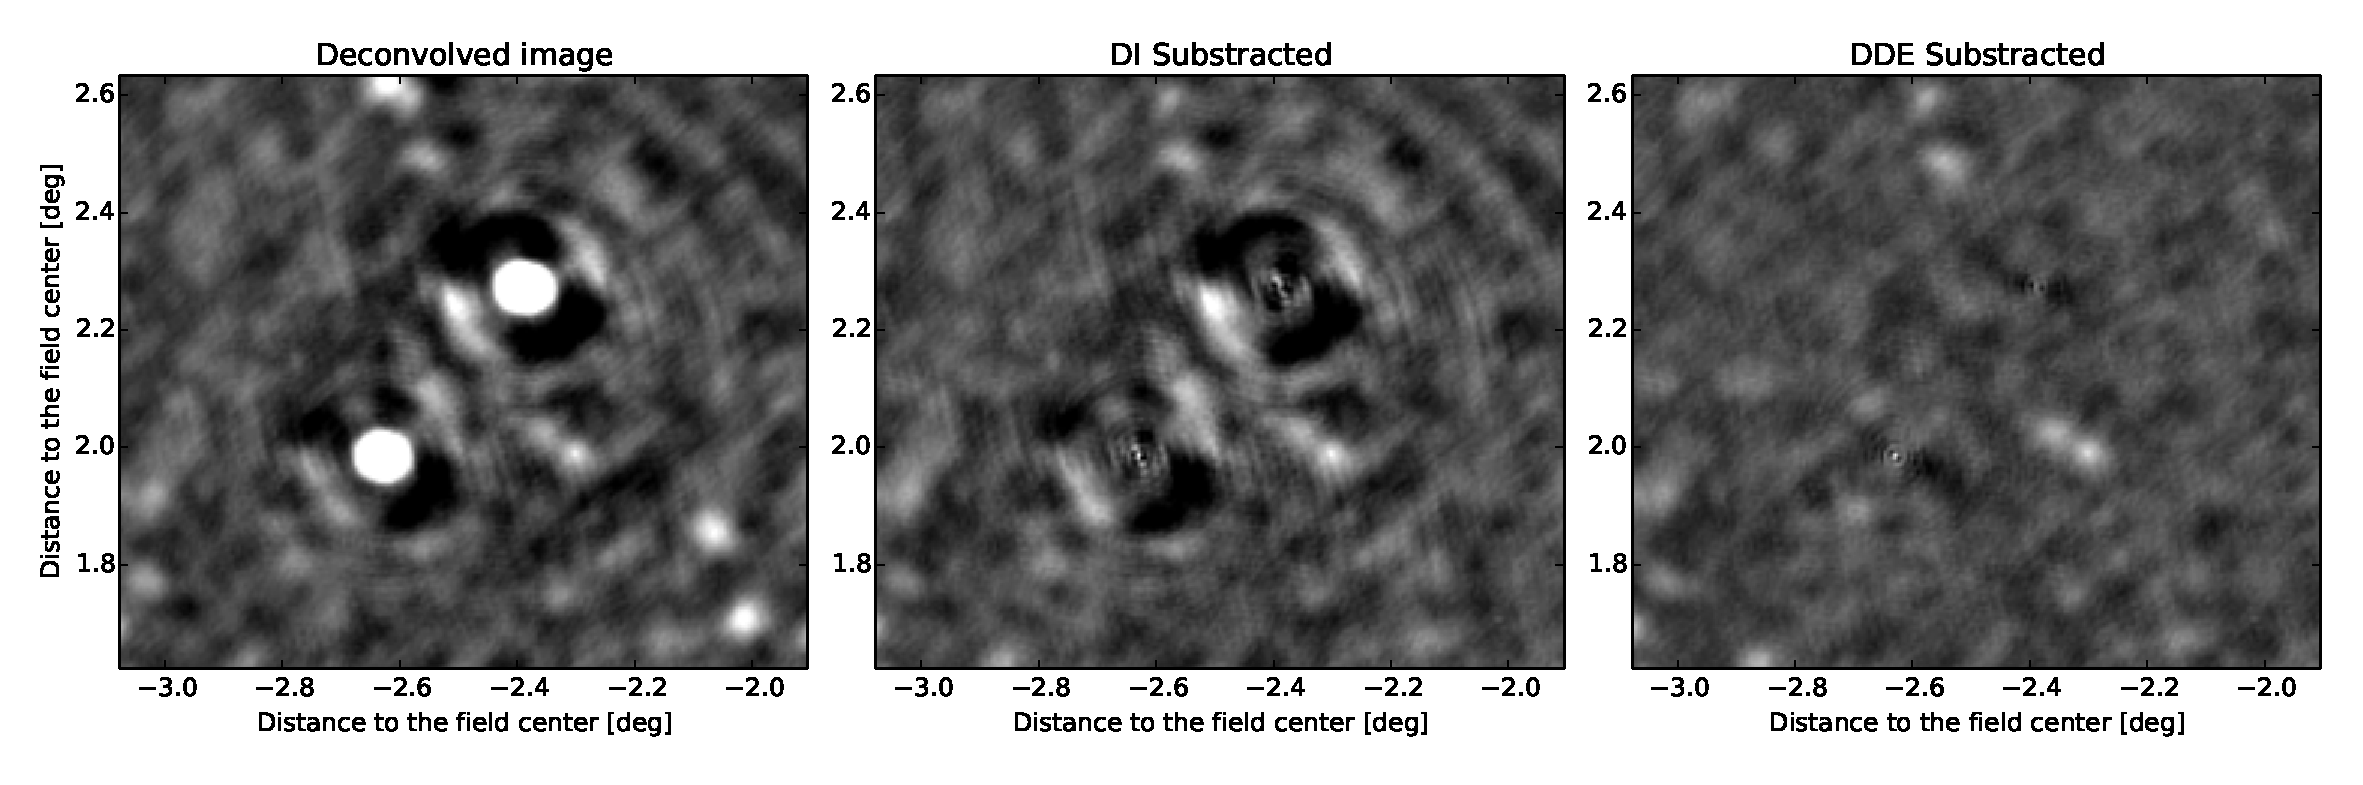
\includegraphics[width=\textwidth]{residZoom}
%% \caption{\label{fig:resid} This figure shows compares the image
%%   (left), the residuals data after simple skymodel substraction
%%   (center), and the residuals data after substracting the
%%   sky model corrupted by the direction-dependent solution (right).}
%% \end{center}
%% \end{figure*}

